\chapter{Incident Sequence and Attack Timeline}
\begin{figure}[H]
\centering
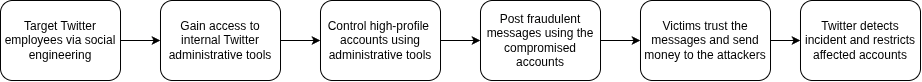
\includegraphics[width=1.0\linewidth]{img/timeline.png}
\caption{Timeline of the incident. Source: Made with draw.io}
\end{figure}
The figure explains the attack timeline of the incident and consists of the following six events:
\begin{enumerate}
\item \textbf{Target Twitter employees via social engineering:} At the first stage of the incident, the attackers targeted Twitter employees via a phone spear phishing attack and obtained their credentials. This step was the initial point of compromise as the attackers not only managed to obtain credentials from Twitter employees, even though these employee accounts were incapable of accessing administrative tools.
\item \textbf{Gain access to Twitter's internal administrative tools:} When the rights of the compromised employee accounts were not sufficient to access Twitter's internal administrative tools, the attackers targeted employees who had access to these tools and managed to retrieve their credentials via additional social engineering. This event is an escalation of the initial point of compromise as the attackers managed to compromise employee accounts that were authorized to use Twitter's internal administrative tools. Additionally, this step is important because when the attackers realized, that the employee accounts they compromised, lacked the rights for the administrative tools, they moved to employees that had the necessary rights. Lastly, the attackers did not exploit any technical vulnerabilities in Twitter's systems but managed to trick employees to give them their credentials instead. 
\item \textbf{Control high-profile accounts using administrative tools:} With the employee accounts with permission to use Twitter's internal administrative tools, the attackers were capable of hijacking the accounts of several high-profile Twitter accounts that included celebrities, politicians as well as companies. In total, the attackers targeted 130 accounts and post messages from 45 of them.
\item \textbf{Post fraudulent messages using the compromised accounts:} With the attackers gaining access to the high-profile accounts, they were able to send messages on Twitter using these accounts. At around 20:00 UTC, messages appeared, claiming that the sender will give double the amount of Bitcoin that a user sends to a designated Bitcoin wallet; often in the context of charity.
\begin{figure}[H]
\centering
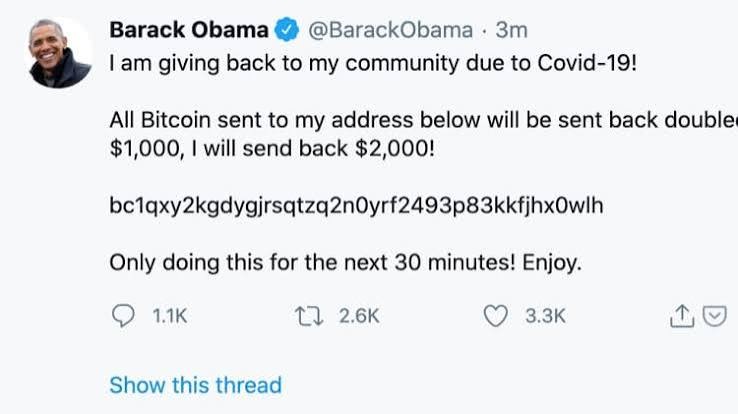
\includegraphics[width=0.5\linewidth]{img/scam.png}
\caption{Example of a message from the attackers pretending to be former US president Barack Obama. Source: CNBC}
\end{figure}
\item \textbf{Victims trust the messages and send money to the attackers:} 
As the attackers sent the messages from verified Twitter accounts from personalities or companies that have the financial capacity to repay double the amount of Bitcoin sent, users believed that the messages were legitimate and sent Bitcoin to the addresses given by the attackers.
\item \textbf{Twitter detects incident and restricts affected accounts:} 
At 21:45 UTC, Twitter detected the incident and posted a statement stating they were aware of the incident and are consequently disabled the ability to send messages from the affected accounts or reset their passwords. Additionally, as the messages followed a similar phrasing pattern, Twitter was able to remove fraudulent messages.
\end{enumerate}